\documentclass[19pt]{beamer}

\usepackage{graphicx}
\usepackage[utf8]{inputenc}
% \usepackage{fontenc}
\usepackage{beamerthemesplit}
\usepackage{xcolor}
\usepackage[OT4]{fontenc}
% \usepackage[polish]{babel}
% \usepackage[utf8]{inputenc}
% \usepackage{ucs}
% \usepackage[MeX]{polski} 
% \usepackage{polski}
% \usepackage{lmodern} 
% \usepackage{fontspec}

% COLORS (Tango)
\definecolor{LightButter}{rgb}{0.98,0.91,0.31}
\definecolor{LightOrange}{rgb}{0.98,0.68,0.24}
\definecolor{LightChocolate}{rgb}{0.91,0.72,0.43}
\definecolor{LightChameleon}{rgb}{0.54,0.88,0.20}
\definecolor{LightSkyBlue}{rgb}{0.45,0.62,0.81}
\definecolor{LightPlum}{rgb}{0.68,0.50,0.66}
\definecolor{LightScarletRed}{rgb}{0.93,0.16,0.16}
\definecolor{Butter}{rgb}{0.93,0.86,0.25}
\definecolor{Orange}{rgb}{0.96,0.47,0.00}
\definecolor{Chocolate}{rgb}{0.75,0.49,0.07}
\definecolor{Chameleon}{rgb}{0.45,0.82,0.09}
\definecolor{SkyBlue}{rgb}{0.20,0.39,0.64}
\definecolor{Plum}{rgb}{0.46,0.31,0.48}
\definecolor{ScarletRed}{rgb}{0.80,0.00,0.00}
\definecolor{DarkButter}{rgb}{0.77,0.62,0.00}
\definecolor{DarkOrange}{rgb}{0.80,0.36,0.00}
\definecolor{DarkChocolate}{rgb}{0.56,0.35,0.01}
\definecolor{DarkChameleon}{rgb}{0.30,0.60,0.02}
\definecolor{DarkSkyBlue}{rgb}{0.12,0.29,0.53}
\definecolor{DarkPlum}{rgb}{0.36,0.21,0.40}
\definecolor{DarkScarletRed}{rgb}{0.64,0.00,0.00}
\definecolor{Aluminium1}{rgb}{0.93,0.93,0.92}
\definecolor{Aluminium2}{rgb}{0.82,0.84,0.81}
\definecolor{Aluminium3}{rgb}{0.73,0.74,0.71}
\definecolor{Aluminium4}{rgb}{0.53,0.54,0.52}
\definecolor{Aluminium5}{rgb}{0.33,0.34,0.32}
\definecolor{Aluminium6}{rgb}{0.18,0.20,0.21}

\hypersetup{
	linkcolor=DarkSkyBlue,
	citecolor= DarkSkyBlue,
	filecolor= DarkSkyBlue,
	urlcolor= DarkSkyBlue
}

% \setmonofont[Scale=0.8]{Liberation Mono}

\DeclareGraphicsExtensions{.pdf,.jpg,.png,.tif}

\AtBeginSection[]{
 \begin{frame}<presentation>[plain]
 \frametitle{Plan prezentacji}
 \tableofcontents[currentsection]
 \end{frame}}

\usetheme{Darmstadt} 
% \usetheme{AnnArbor}
% \usecolortheme{beetle}

\usepackage{listings}
\usepackage{color}

\title{Z Rails do Merba i... z powrotem}
\author{Marcin Kulik, Piotr Solnica}
\date{13/01/2009, KRUG, Lunar Logic Polska}

\lstset{language=ruby}
\lstset{stepnumber=2, tabsize=2, showstringspaces=false}
\lstset{backgroundcolor=\color{white}}
% keywordstyle=\color{orange}\bfseries, identifierstyle=\color{blue}, stringstyle=\color{green}}
% \lstset{otherkeywordstyle=\color{yellow}, numberstyle=\color{red}}
% \lstset{otherkeywordsstyle=\color{yellow}, numbersstyle=\color{red}}
% \lstset{morekeywordstyle=\color{yellow}}
% \lstset{morekeywordsstyle=\color{yellow}}

\lstset{
	keywordstyle=[1]{\color{DarkSkyBlue}},
	keywordstyle=[2]{\color{DarkScarletRed}},
	keywordstyle=[3]{\bfseries},
	keywordstyle=[4]{\color{DarkPlum}},
	keywordstyle=[5]{\color{SkyBlue}},
	commentstyle={\color{Aluminium4}},
	stringstyle={\color{Chocolate}},
	basicstyle={\tiny\ttfamily},
}
\begin{document}
\begin{center}

\frame{\titlepage}

\section[Outline]{}
\frame{\tableofcontents}

\section{Wprowadzenie}
\subsection{Na początku był Rubytime}

\begin{frame}
Jest 2005 rok

Rails to nowość
\end{frame}

\begin{frame}
LLP potrzebuje systemu do timetrackingu

Powstaje Rubytime 1
\end{frame}

\begin{frame}
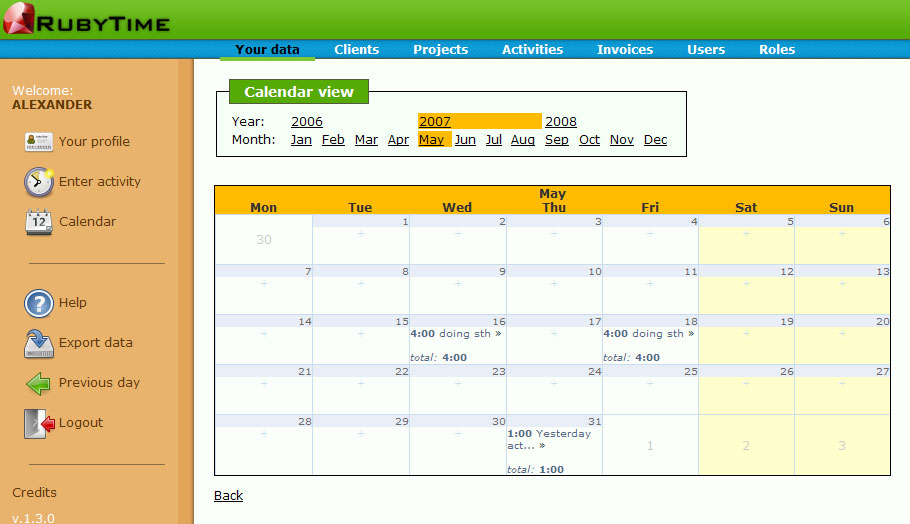
\includegraphics[width=1.0\textwidth]{rt1.jpg} 
\end{frame}

\begin{frame}
Rubytime 2 jako naturalne przedłużenie wersji 1

Nadal Rails
\end{frame}

\subsection{Rodzi się "konkurencja"}

\begin{frame}
W między czasie powstają:
\begin{itemize}
\item Ramaze
\item Mack
\item Sinatra
\item Camping
\item Merb
\end{itemize}
\end{frame}

%\lstinputlisting{merb1.rb}

\begin{frame}
Jednak Rails nadal "bezkonkurencyjny":
\begin{itemize}
\item największy userbase spośród wymienionych
\item coraz więcej literatury
\item coraz łatwiejsze hostowanie (Passenger)
\end{itemize}
\end{frame}

\begin{frame}
Ale czy napewno jedyny liczący się framework dla Ruby'ego? Niekoniecznie!
\end{frame}

\subsection{Rubytime 3}

\begin{frame}
Potrzeba "odświeżenia" RT

+ 

zbliżający się wielkimi krokami Merb 1.0 

= 

Rubytime 3
\end{frame}

\begin{frame}
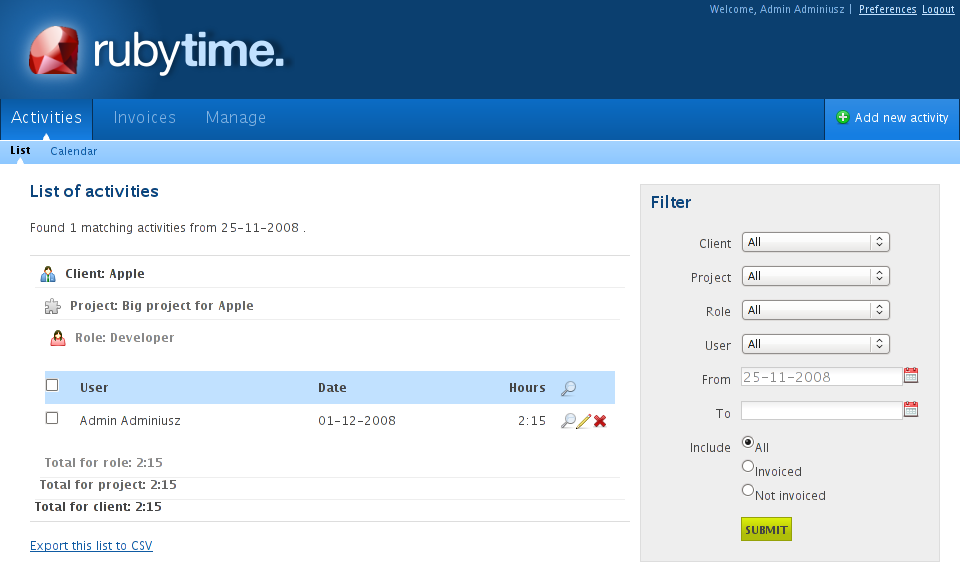
\includegraphics[width=1.0\textwidth]{rt-full.png} 
\end{frame}

\begin{frame}
Wrażenia?

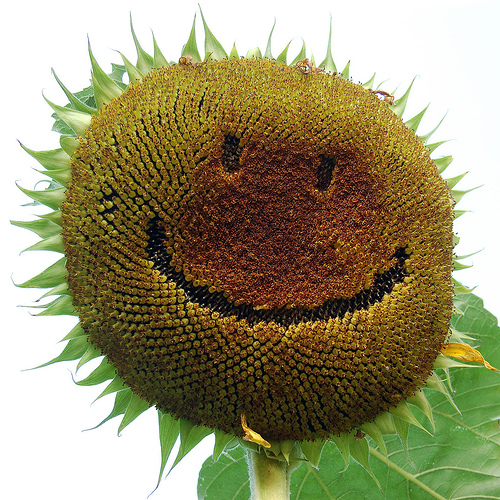
\includegraphics[width=0.6\textwidth]{sloneczki.jpg} 
\end{frame}

\subsection{I ponownie Rails}

\begin{frame}
Merb łączy się z Rails ?!
\end{frame}

\begin{frame}
Rails 2.3 ewoluuje w kierunku Rails 3

Merb 1.0 ewoluuje w kierunku Merb 2

Merb 2 == Rails 3
\end{frame}

\section{Merb}

\subsection{Założenia Merba}

\begin{frame}
Szybkość i zużycie pamięci:
\begin{itemize}
\item No code is faster than no code (Call stack w Rails to 41-58 wywołań, w Merb 27-32 wywołań)
\item Wszystko co spowalnia Merba jest bugiem
\item Rails 24K-50K LOC, Merb 10K-17K LOC
\item Bez magicznych sztuczek (alias\_method\_chain, method\_missing itp wypadają...)
\end{itemize}
\end{frame}

\begin{frame}
Elastyczność
\begin{itemize}
\item ORM (DataMapper, ActiveRecord, Sequel...)
\item Javascript library (jQuery, Prototype...)
\item Testowanie (unit, rspec...)
\item Template engine (erb, haml...)
\end{itemize}
\end{frame}

\begin{frame}
Modularność ("nie, nie potrzebujesz wszystkiego")
\begin{itemize}
\item Rails 6 gemów
\item Merb 18 (core + more)
\end{itemize}
\end{frame}

\begin{frame}
Stabilne publicze API i pluginy
\begin{itemize}
\item API miało się nie zmieniać dla wersji major, czas pokaże
\item pluginy to Gemy
\item zapewniają zależności
\item korzystają z API zamiast opierać się na ciągle zmieniających się metodach prywatnych
\end{itemize}
\end{frame}

\begin{frame}
Rack
\begin{itemize}
\item odpowiednik Pythonowego WSGI czy Javowego Servlet API
\item nie przywiązuje aplikacji do konkretnego serwera
\item obsługa w Passenger
\end{itemize}
\end{frame}

\begin{frame}
Generowanie aplikacji
\begin{itemize}

\item fullstack: merb-gen app
\item core: merb-gen core
\item simple: merb-gen flat
\item single-file: merb-gen very\_flat

\end{itemize}

\end{frame}

\subsection{Router}

\begin{frame}
Router

\lstinputlisting{merb-router.rb}
\end{frame}

\subsection{Kontrolery}

\begin{frame}
provides + display + render

\lstinputlisting{merb-display.rb}
\end{frame}

\begin{frame}
Przetwarzanie w tle

\lstinputlisting{merb-run.rb}
\end{frame}

\begin{frame}
Asset bundling

\lstinputlisting{merb-assets.rb}
\end{frame}

\begin{frame}
Wyjątki:

raise NotFound odpali: kontroler Exceptions, akcja :not\_found, status 404
\end{frame}

\begin{frame}
action-args

\lstinputlisting{merb-actionargs.rb}
\end{frame}

\subsection{Slices}

\begin{frame}

\includegraphics[width=0.8\textwidth]{dawg.png} 
\end{frame}

\begin{frame}
Slice = aplikacja w aplikacji, zawiera własne:
\begin{itemize}
\item kontrolery, 
\item model, 
\item widoki 
\item routes'y
\end{itemize}
\end{frame}

\begin{frame}
merb-auth = "restful\_authentication done right"
\end{frame}

\subsection{Parts}

\section{Skutki połączenia Merb z Rails}
\subsection{Na plus}

\begin{frame}
Pozytywne aspekty połączenia:
\begin{itemize}
\item większy Rails core-team (Merb core-team to mądrzy goście)
\item router oraz bootloader Merb w Rails (prace już trwają)
\end{itemize}
\end{frame}

\begin{frame}
Pozytywne aspekty połączenia:
\begin{itemize}
\item respond\_as/respond\_with jako odpowiednik merbowych provides i display (prace już trwają)
\item Rails mają zyskąc slice'y, jeszcze lepsze niz były w Merbie
\item czyszczenie kodu
\end{itemize}
\end{frame}

\subsection{Na minus}

\begin{frame}
Negatywne aspekty połączenia:
\begin{itemize}
\item brak poważnej konkurencji = mniejsze tempo rozwoju
\item DHH.. Czy współpraca z Davidem przyniesie zakładane wyniki?
\end{itemize}
\end{frame}

\section{The End}

\begin{frame}
Dziękuję. Pytania?
\end{frame}

\end{center}
\end{document} 